\subsubsection*{Descartes / Catesian Coordinate}

$$\raisebox{-0.5\height}{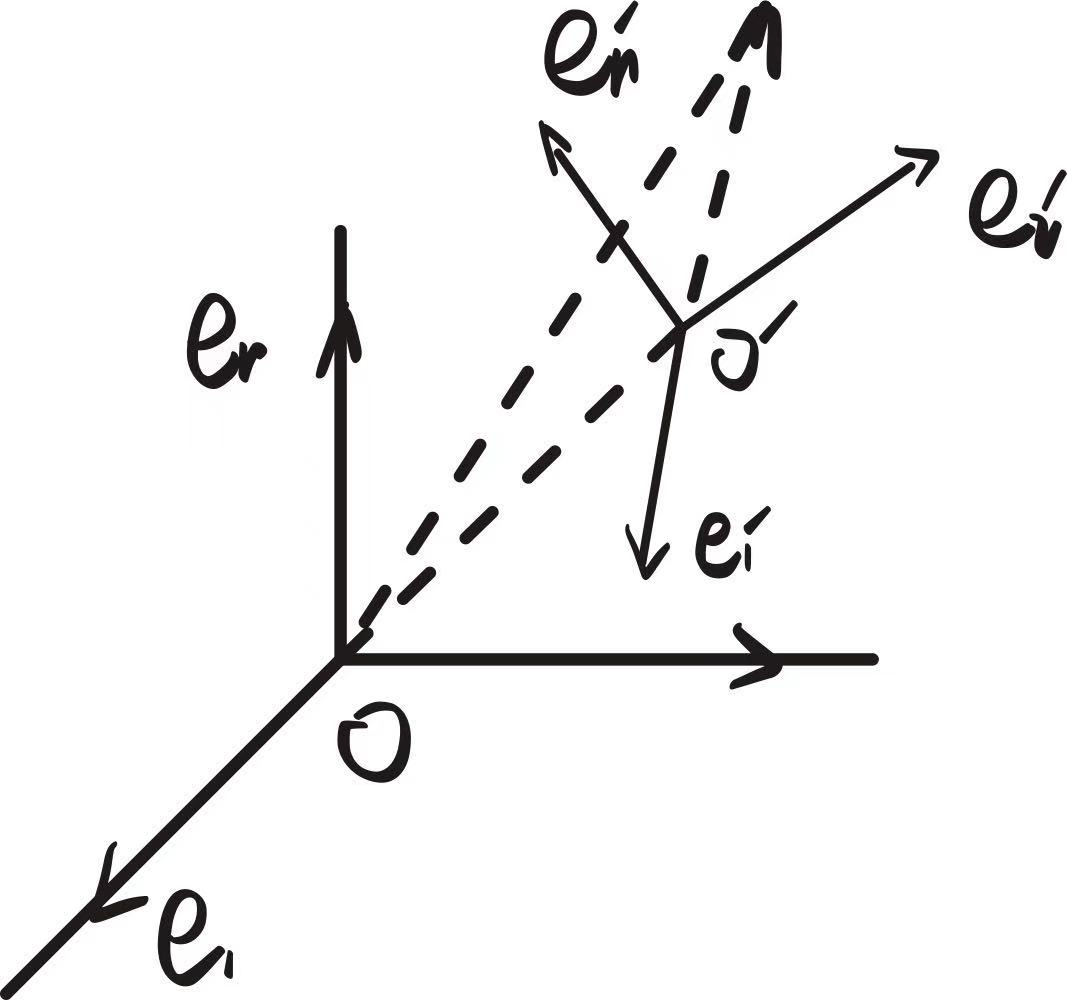
\includegraphics[height=3cm]{chapters/08/D-CC}}
    \mathbb{F}\left[0';\underbrace{e_1',\dots,e_n'}_{\substack{\begin{pmatrix}e_1'&\cdots&e_n'\end{pmatrix}=\begin{pmatrix}e_1'&\cdots&e_n'\end{pmatrix}P\\P\in O(n)}}\right]
$$
A point has coordinate
\begin{align*}\begin{cases}
                                \overrightarrow{x'}=\begin{pmatrix}
                                x_1'   \\
                                \vdots \\
                                x_n'
                            \end{pmatrix}\text{ in }\mathbb{F}\left[0';e_1',\dots,e_n'\right] \\
                                \overrightarrow{x}=\begin{pmatrix}
                               x_1    \\
                               \vdots \\
                               x_n
                           \end{pmatrix}\text{ in }\mathbb{F}\left[0;e_1,\dots,e_n\right]
                            \end{cases} & \implies\underset{=\left(
                  e_1\cdots e_n
              \right)\overrightarrow{v}}{\overrightarrow{OO'}}+\begin{pmatrix}
                                                                   e_1' & \cdots & e_n'
                                                               \end{pmatrix}\overrightarrow{x'}=\begin{pmatrix}
                                                                                                    e_1 & \cdots & e_n
                                                                                                \end{pmatrix}\overrightarrow{x}                                           \\
                                                                                                                   & \implies\overrightarrow{x}=\overrightarrow{v}+p\overrightarrow{x'}
\end{align*}

\begin{enumerate}[label={Step \arabic*.}]
    \item $\overrightarrow{x}=p\overrightarrow{x'}\implies x'\underset{\text{对角阵}}{P^TAP}x'+b^TPx'+c=0$

          Find $P$ s.t.$$\xrightarrow{\text{\textbf{orthogonal diagaloization}}}P^TAP=\Lambda=\operatorname{diag}\left(\lambda_1,\dots,\lambda_{r_+},-\lambda_{r_++1},\dots,-\lambda_{r_++r_-},\underbrace{0,\dots,0}_{n-\operatorname{rank}A}\right)$$
          then $\lambda_1x_1'^2+\dots+\lambda_{r_+}x_{r_+}'^2-\lambda_{r_++1}x_{r_++1}'^2-\dots-\lambda_{r_++r_-}x_{r_++r_-}'^2+\mathbf{b_1'x_1'+\dots+b_n'x_n'}+c=0$
    \item Completing square for the variables $x_1',\dots,x_{r_+}',x_{r_++1}',\dots,x_{r_++r_-}'$
          $$\begin{pmatrix}
                  x_1'         \\
                  \vdots       \\
                  x_{r_+}'     \\
                  x_{r_++1}'   \\
                  \vdots       \\
                  x_{r_++r_-}' \\
                  \vdots       \\
                  x_n'
              \end{pmatrix}=\begin{pmatrix}
                  x_1''-\frac{b_1'}{2\lambda_1}                         \\
                  \vdots                                                \\
                  x_{r_+}''-\frac{b_{r_+}'}{2\lambda_v}                 \\
                  x_{r_++1}''-\frac{b_{r_++1}'}{2\lambda_{r_++1}}       \\
                  \vdots                                                \\
                  x_{r_++r_-}''-\frac{b_{r_++r_-}'}{2\lambda_{r_++r_-}} \\
                  x_{r_++r_-+1}''                                       \\
                  \vdots                                                \\
                  x_n''
              \end{pmatrix}$$
          i.e. $x_1'=x''+b''$
          $$\lambda_1x_1''^2+\dots+\lambda_{r_+}x_{r_+}''^2-\lambda_{r_++1}x_{r_++1}''^2-\dots-\lambda_{r_++r_-}x_{r_++r_-}''^2+b_{r_++r_-+1}'x_{r_++r_-+1}''+\dots+b_n'x_n''+c=0$$
    \item Case 1.$$b_{r+1}'=\dots=b_n'=0\leadsto x''^T\operatorname{diag}\left(\lambda_1,\dots,\lambda_{r_+},-\lambda_{r_++1},\dots,-\lambda_{r_++r_-},0,\dots,0\right)x''+c=0$$
          Case 2. We can do another orthogonal transformation on the variable $x_{r+1}'',\dots x_n''$ to simplify the 1st-order term s.t. the 1st order term brcomes $b_{r+1}'''x_{r+1}'''$
\end{enumerate}

Back to plane in $\mathbb{R}^3$: $ax+by+cz+d=0$\raisebox{-0.5\height}{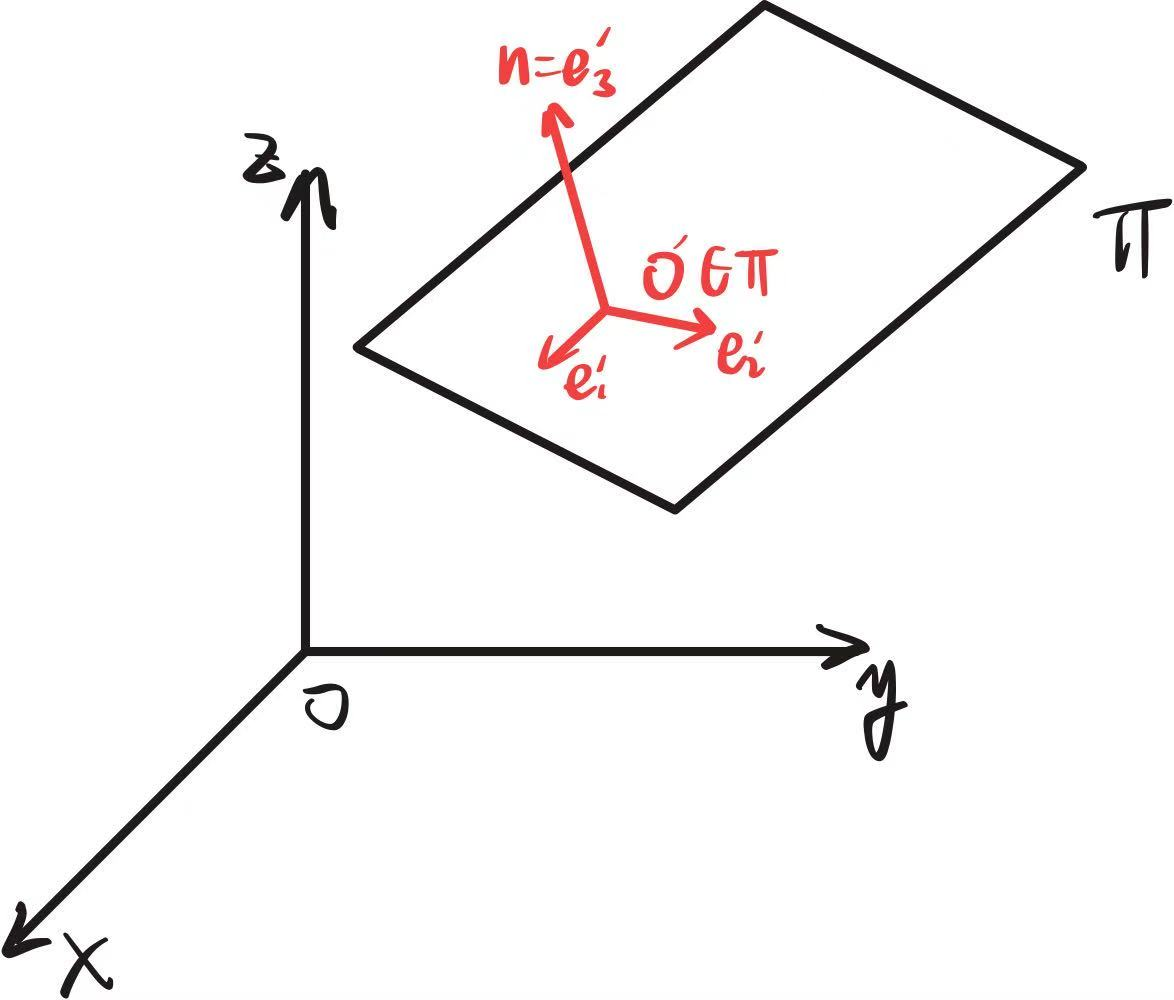
\includegraphics[height=3cm]{chapters/08/axbyczd0}}

\allbold{Let $e_3'=n=\frac{(a,b,c)}{\sqrt{a^2+b^2+c^2}}$, $e_1',e_2'$ parallel to $\Pi$ s.t. $\left(e_1',e_2',n\right)$ is an orthonormal basis, then in the Cartesian coordinate $\mathbb{F}\left[0';e_1',e_2',e_3'\right]$, $\Pi$ is defined by \emph{$z'=0$}}

\emph{$$\begin{pmatrix}
            a & b & c
        \end{pmatrix}\begin{pmatrix}
            x \\y\\z
        \end{pmatrix}+d=0
    $$
    Let $\begin{pmatrix}
            x \\y\\z
        \end{pmatrix}=P\begin{pmatrix}
            x' \\y'\\z'
        \end{pmatrix}+q$ (Euclidean transformation), then the equation is changed to
    $$\begin{pmatrix}
            a & b & c
        \end{pmatrix}P\begin{pmatrix}
            x' \\y'\\z'
        \end{pmatrix}+\begin{pmatrix}
            a & b & c
        \end{pmatrix}q+d=0$$
    find $P\in O(3),\,q\in\mathbb{R}^3$ s.t. $\begin{pmatrix}
            a & b & c
        \end{pmatrix}P=\begin{pmatrix}
            0 & 0 & c
        \end{pmatrix},\,c\neq 0,\,\begin{pmatrix}
            a & b & c
        \end{pmatrix}q+d=0$}

\begin{thm}
    Given $S=\left\{\overrightarrow{x}\in\mathbb{R}^n\mid f\left(\overrightarrow{x}\right)=\overrightarrow{x}^TA\overrightarrow{x}+\overrightarrow{b}^T\overrightarrow{x}+c=0\right\}$, we can find a coordinate transformation of the form $\overrightarrow{x}=P\overrightarrow{y}+\overrightarrow{a}$, where $P\in SO(n)=\left\{Q\in O(n)\mid\det{Q}=1\right\}$ and $\overrightarrow{q}\in\mathbb{R}^n$, such that the equation $f\left(\overrightarrow{x}\right)=0$ becomes
    \begin{enumerate}[label=(\arabic*)]
        \item $\sum_{i=1}^{r_+}\lambda_iy_i^2-\sum_{j=r_++1}^{r_++r_-}\lambda_jy_j^2=c$ or
        \item $\sum_{i=1}^{r_+}\lambda_iy_i^2-\sum_{j=r_++1}^{r_++r_-}\lambda_jy_j^2-y_{r_++r_-+1}=0$
    \end{enumerate}
\end{thm}